\chapter{Results}
\label{ch:results}

This chapter presents the results of our model training and evaluation. After building and tuning Decision Tree, K-Nearest Neighbors (KNN), and Random Forest regressors using ZIP-based splits, we assessed how well each model predicted year-over-year home value growth. Results are shown across three key areas: model performance with different feature counts, test set prediction accuracy, and model behavior over time for a sample ZIP code.

\section{Feature selection and model comparison}

We first examined how the number of selected features affected each model's performance. For every value of $k$ from 1 to 50, we used both f-regression and mutual information to rank features. The top-$k$ features were then used to compute 3-fold cross-validated $R^2$ scores for each model.

\begin{figure}[!ht]
    \centering
    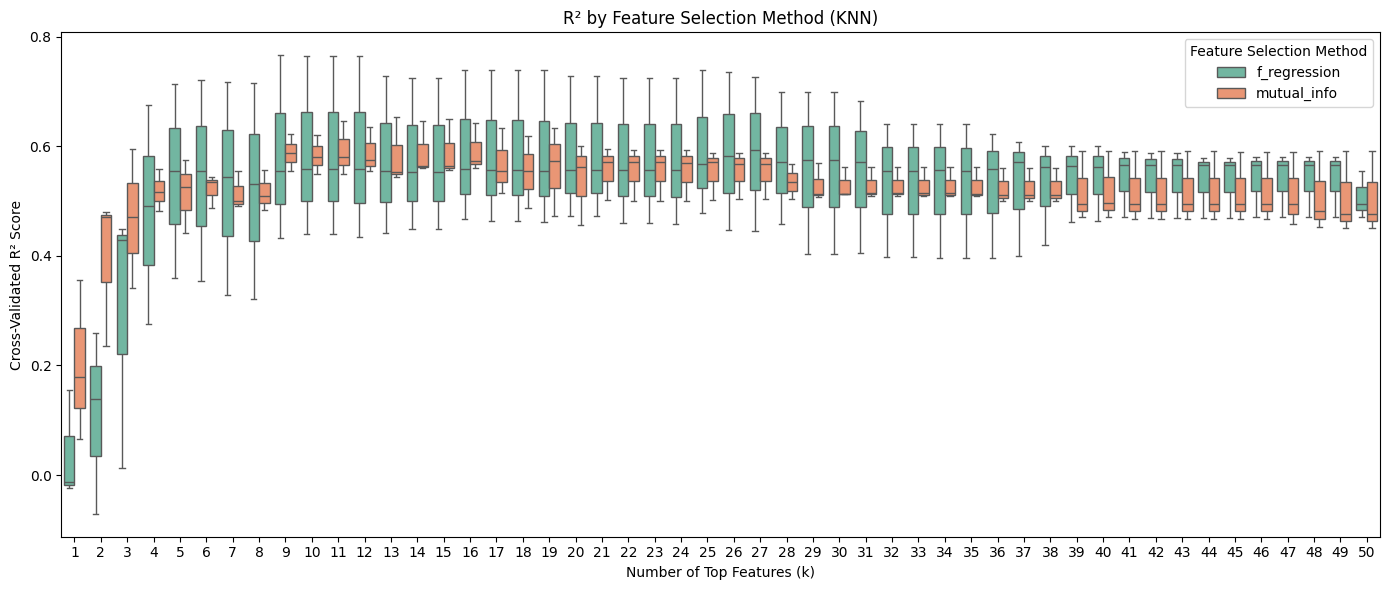
\includegraphics[width=\textwidth]{figures/box50_KNN.png}
    \caption{Cross-validated $R^2$ scores for KNN model.}
    \label{fig:box_knn}
\end{figure}
\FloatBarrier

In Figure~\ref{fig:box_knn}, the KNN model shows a clear performance increase up to about 8 or 9 features, after which the $R^2$ scores plateau. f-regression consistently led to slightly higher performance at low values of $k$, with mutual information catching up as more features were added. Beyond 12–15 features, there was no significant improvement, and some increase in variance was observed, especially with mutual information.

\begin{figure}[!ht]
    \centering
    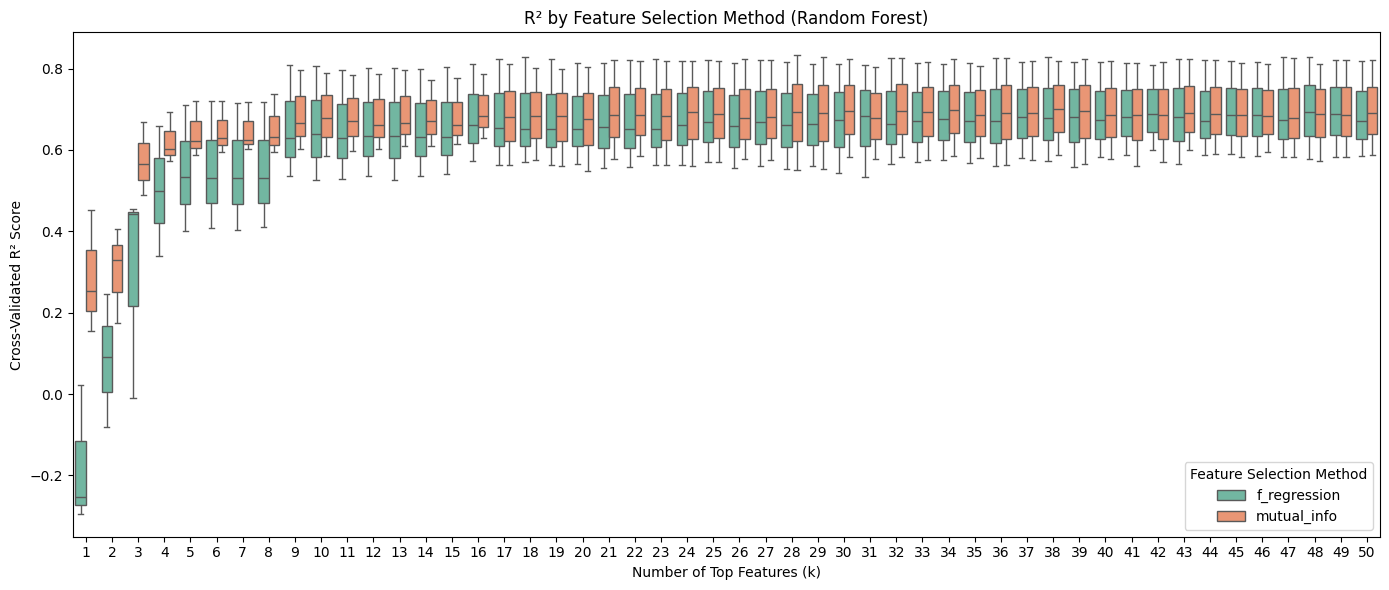
\includegraphics[width=\textwidth]{figures/box50_RF.png}
    \caption{Cross-validated $R^2$ scores for Random Forest model.}
    \label{fig:box_rf}
\end{figure}
\FloatBarrier

Random Forest results in Figure~\ref{fig:box_rf} show a steep improvement in $R^2$ from 1 to around 15 features, peaking between 15–20 features. After that, performance remains mostly stable. The model is more robust to the number of features used, with mutual information providing slightly more consistent results at higher $k$. The box plots are compact throughout, indicating stable behavior across folds.

\begin{figure}[!ht]
    \centering
    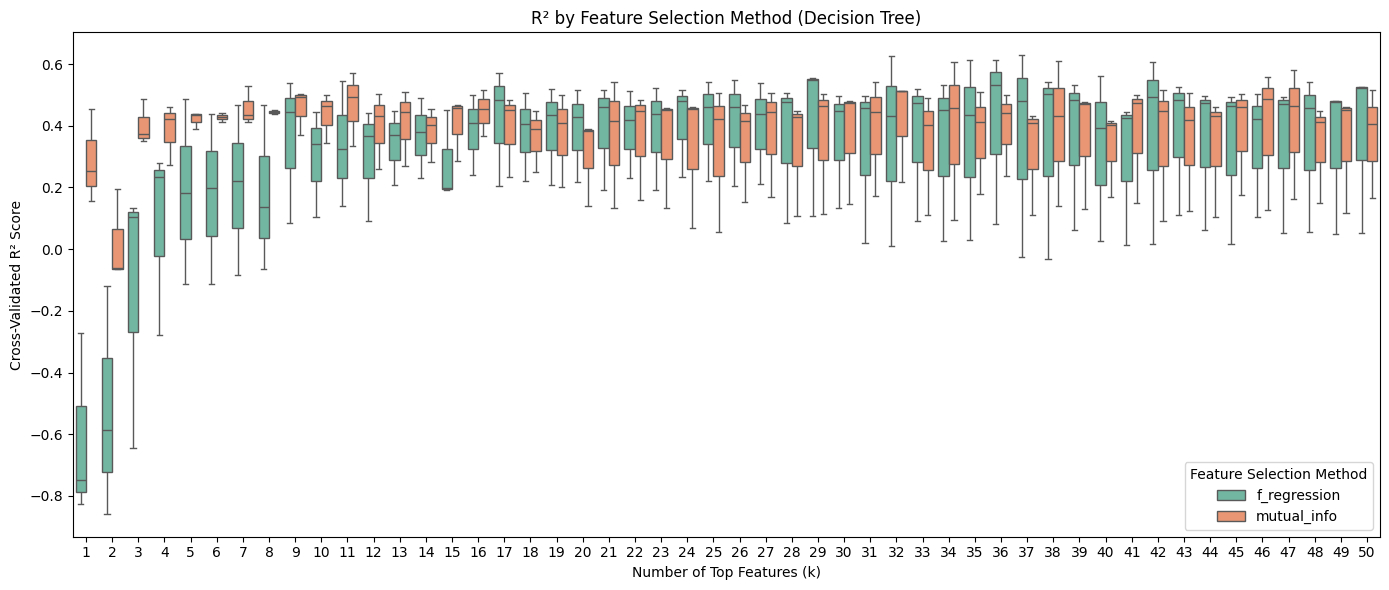
\includegraphics[width=\textwidth]{figures/box50_DT.png}
    \caption{Cross-validated $R^2$ scores for Decision Tree model.}
    \label{fig:box_dt}
\end{figure}
\FloatBarrier

Figure~\ref{fig:box_dt} shows that the Decision Tree model is the most sensitive to the number of features. Performance improves up to around 8–10 features, but quickly deteriorates beyond that, especially with mutual information. This is likely due to overfitting. The most compact and stable results occurred when using 8–12 features, with f-regression performing slightly better overall.

Based on these observations, we selected the following number of features for each model:
\begin{itemize}
    \item \textbf{Decision Tree:} 8 features
    \item \textbf{KNN:} 9 features
    \item \textbf{Random Forest:} 16 features
\end{itemize}

\section{Test set prediction accuracy}

We evaluated each model on a held-out test set of ZIP codes that were not used during training. Figures~\ref{fig:rf_pred}, \ref{fig:knn_pred}, and \ref{fig:dt_pred} show the predicted vs actual year-over-year growth values, along with a regression line, an ideal line ($y = x$), and ±1 RMSE bands.

\begin{figure}[!ht]
    \centering
    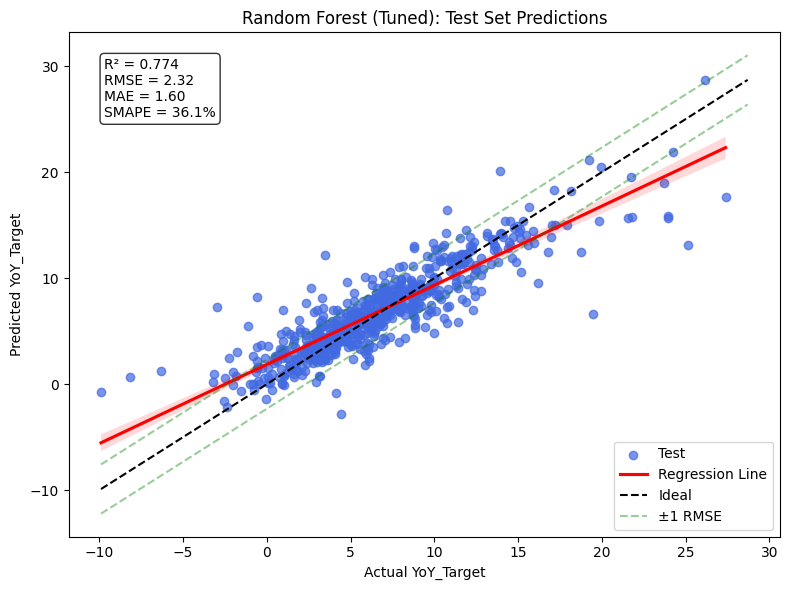
\includegraphics[width=0.75\textwidth]{figures/RF1.png}
    \caption{Random Forest (Tuned): Test set predictions.}
    \label{fig:rf_pred}
\end{figure}
\FloatBarrier

In Figure~\ref{fig:rf_pred}, the Random Forest model shows the strongest test performance. Most predictions fall close to the ideal line, and the regression line closely matches it with a steep slope. The green dashed bands (±1 RMSE) are relatively tight, covering most of the distribution. The model achieved an $R^2$ score of 0.774 on the test set.

\begin{figure}[!ht]
    \centering
    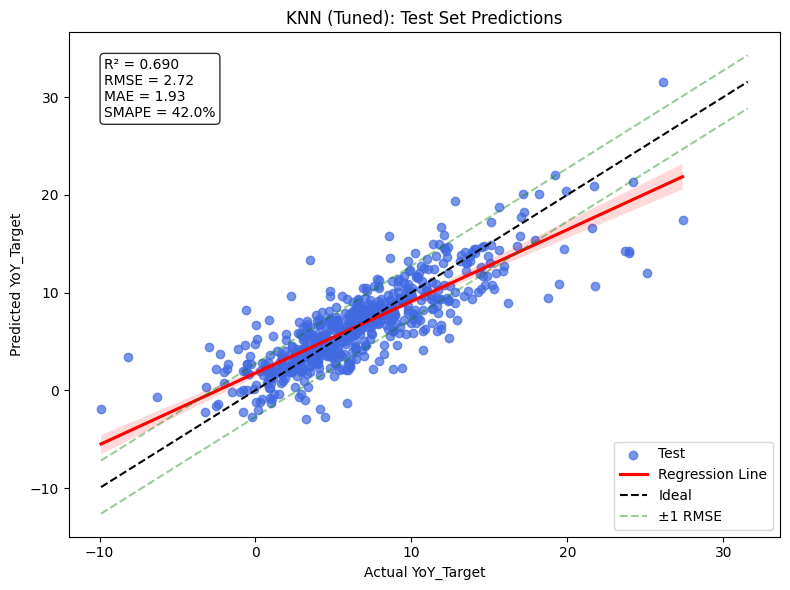
\includegraphics[width=0.75\textwidth]{figures/KNN1.png}
    \caption{KNN (Tuned): Test set predictions.}
    \label{fig:knn_pred}
\end{figure}
\FloatBarrier

The KNN model in Figure~\ref{fig:knn_pred} also performed well, achieving a test $R^2$ of 0.739. Its predictions were slightly more spread out compared to Random Forest, and the regression line was less steep. A few outliers at the higher end of the target range were underpredicted, but the overall alignment to the ideal trend was solid.

\begin{figure}[!ht]
    \centering
    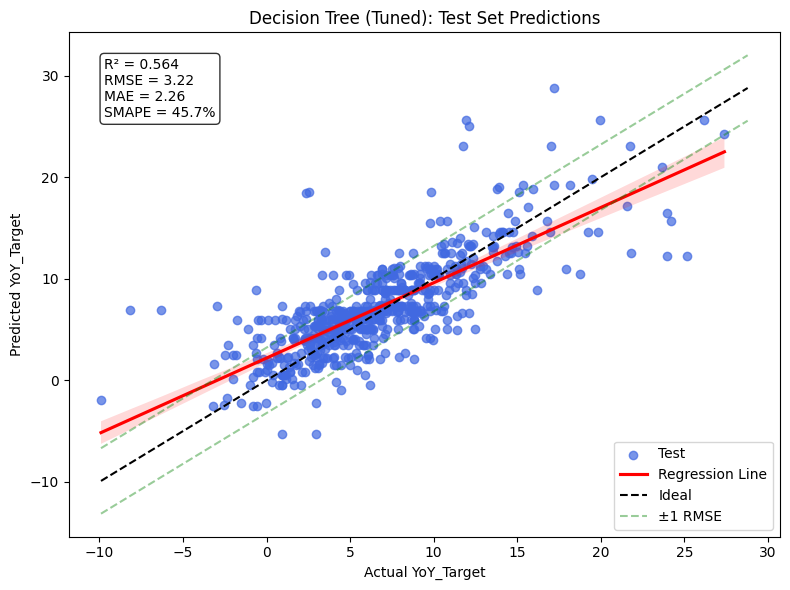
\includegraphics[width=0.75\textwidth]{figures/DT1.png}
    \caption{Decision Tree (Tuned): Test set predictions.}
    \label{fig:dt_pred}
\end{figure}
\FloatBarrier

Figure~\ref{fig:dt_pred} shows the weakest test performance, from the Decision Tree model. Its regression line is noticeably flatter than the ideal, and predictions show more deviation. It underpredicts many higher values and compresses the range of outputs. The test $R^2$ was 0.564, indicating limited generalization.

\section{Train vs test comparison}

To understand how well each model generalizes, we compared train vs test predictions side by side. Figures~\ref{fig:rf_train_test}, \ref{fig:knn_train_test}, and \ref{fig:dt_train_test} show both sets of predictions in one plot.

\begin{figure}[!ht]
    \centering
    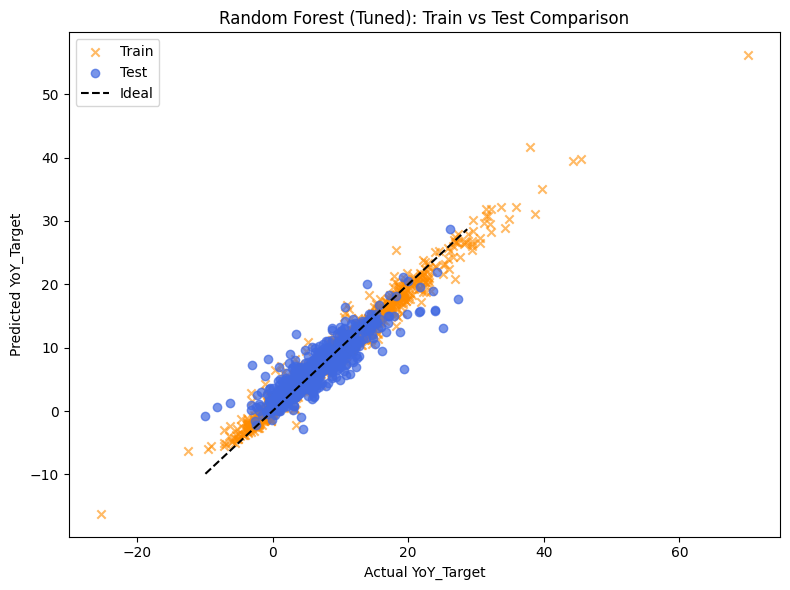
\includegraphics[width=0.75\textwidth]{figures/RF2.png}
    \caption{Random Forest: Train vs test predictions.}
    \label{fig:rf_train_test}
\end{figure}
\FloatBarrier

Figure~\ref{fig:rf_train_test} shows a well-balanced fit for Random Forest. Predictions on both train and test sets are tightly clustered around the ideal line, suggesting the model generalizes well without overfitting.

\begin{figure}[!ht]
    \centering
    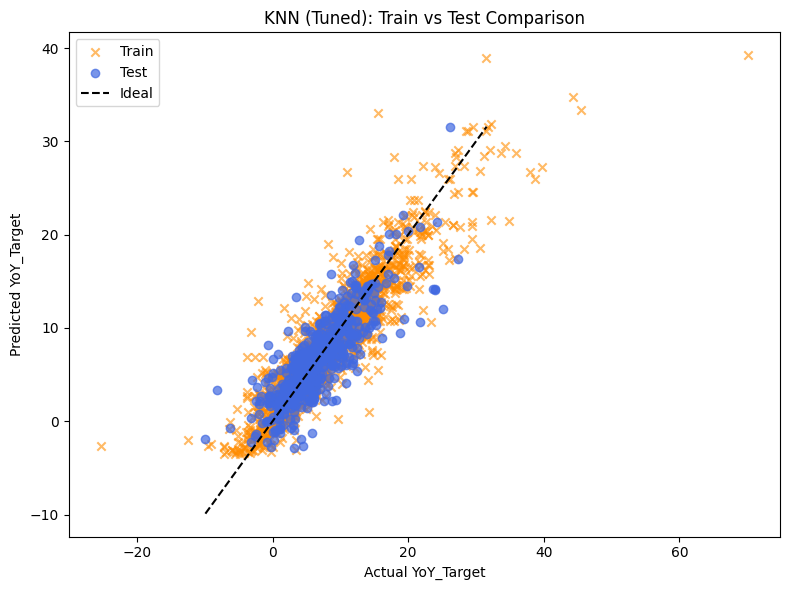
\includegraphics[width=0.75\textwidth]{figures/KNN2.png}
    \caption{KNN: Train vs test predictions.}
    \label{fig:knn_train_test}
\end{figure}
\FloatBarrier

KNN (Figure~\ref{fig:knn_train_test}) also performs consistently across train and test splits, though train predictions are slightly tighter. The test distribution shows slightly more spread, but no major signs of overfitting.

\begin{figure}[!ht]
    \centering
    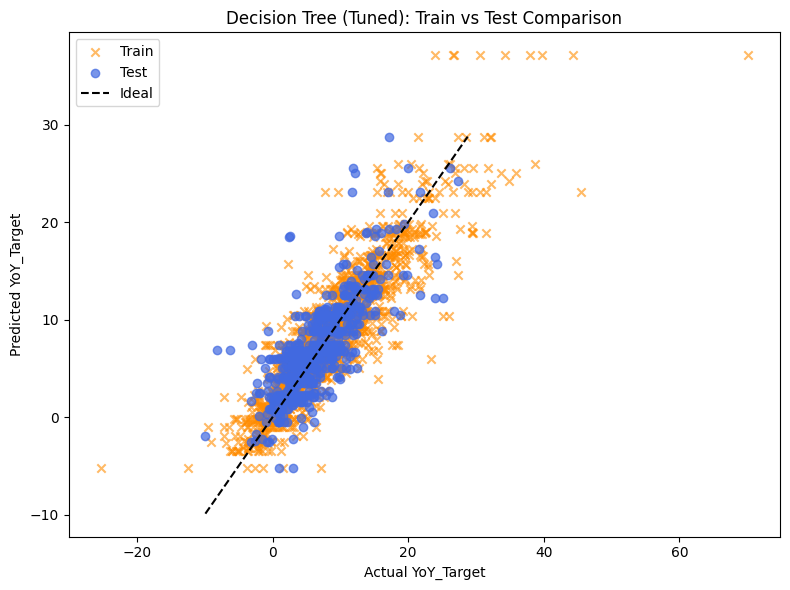
\includegraphics[width=0.75\textwidth]{figures/DT2.png}
    \caption{Decision Tree: Train vs test predictions.}
    \label{fig:dt_train_test}
\end{figure}
\FloatBarrier

The Decision Tree (Figure~\ref{fig:dt_train_test}) shows a stronger fit on the train set than on the test set, with the test predictions exhibiting more variance. This difference suggests some overfitting, consistent with its lower $R^2$ on unseen ZIPs.

\section{Prediction trend over time}

To visualize how each model performs across years for the same location, we selected a ZIP code (31052) and plotted predictions alongside actual YoY values over time.

\begin{figure}[!ht]
    \centering
    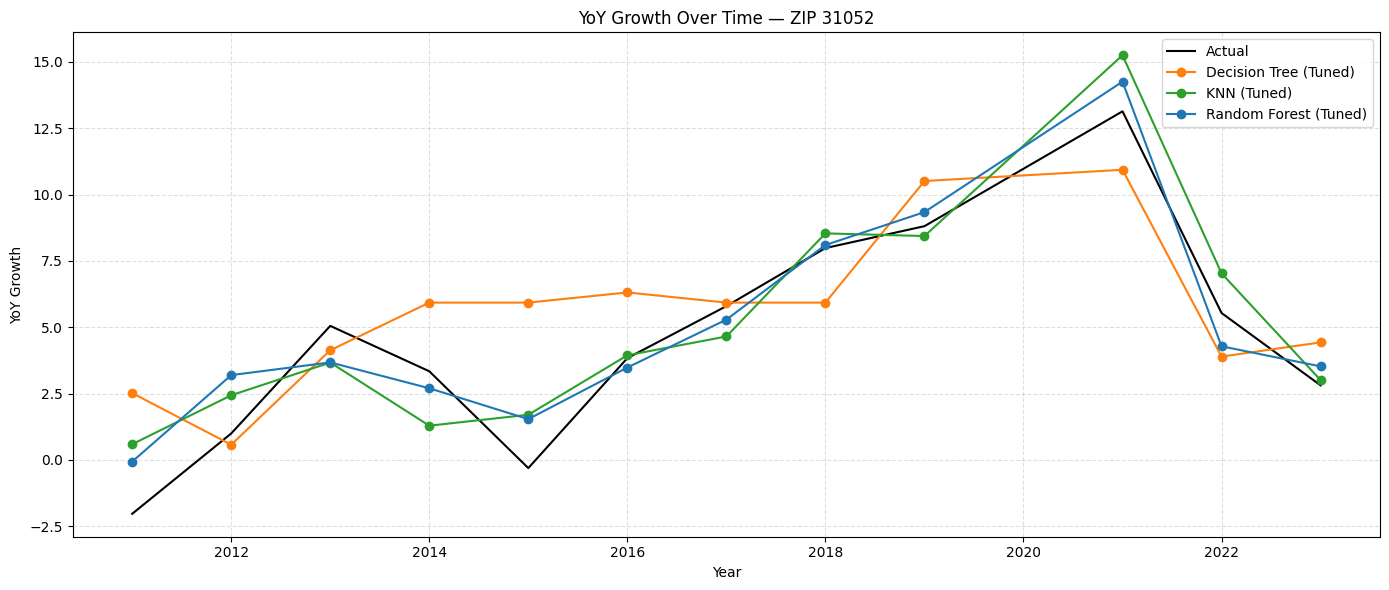
\includegraphics[width=\textwidth]{figures/testpred.png}
    \caption{Predicted vs actual YoY growth over time for ZIP 31052.}
    \label{fig:testpred_zip}
\end{figure}
\FloatBarrier

Figure~\ref{fig:testpred_zip} shows that all models followed the general trend of actual YoY growth, but with different levels of accuracy. Random Forest consistently tracked peaks and dips, while Decision Tree predictions were flatter and missed several changes. KNN captured sharp increases fairly well but overshot in some years. All three models produced usable forecasts, though Random Forest offered the most precise temporal behavior.

\section{Summary of test performance}

Table~\ref{tab:model_results} summarizes final performance on the test set using the selected number of features.

\begin{table}[!ht]
    \centering
    \caption{Model performance on test set (selected features)}
    \label{tab:model_results}
    \begin{tabular}{lcccc}
        \toprule
        \textbf{Model} & \textbf{R\textsuperscript{2}} & \textbf{RMSE} & \textbf{MAE} & \textbf{SMAPE} \\
        \midrule
        Random Forest (16 features) & 0.774 & 2.32 & 1.60 & 36.1\% \\
        KNN (9 features)            & 0.739 & 2.49 & 1.75 & 39.8\% \\
        Decision Tree (8 features) & 0.564 & 3.22 & 2.26 & 45.7\% \\
        \bottomrule
    \end{tabular}
\end{table}
\FloatBarrier

\section{Summary}

All three models captured short-term housing value growth with varying levels of accuracy. Random Forest performed the best across the board, showing strong generalization and tight error margins. KNN followed closely and was relatively stable, but more sensitive to feature selection. Decision Tree required careful tuning and showed signs of overfitting at higher feature counts.

Using both f-regression and mutual information helped ensure that selected features were consistently informative. The ZIP-based split offered a realistic test scenario, ensuring that models were evaluated on truly unseen locations.
